\documentclass[twocolumn]{revtex4}
%\documentclass[onecolumn,12pt]{revtex4}
%\usepackage{amsfonts,amssymb,amsmath,mathbbol}              % for math symbols.
%\usepackage{epstopdf}
%\usepackage{mathbbol}              % for math symbols.
\usepackage{graphics,graphicx,epsfig,ulem} 
\usepackage{amsmath}
\usepackage{multirow}
\usepackage{gensymb}
\usepackage{commath}
\usepackage{textcomp}
\newcommand{\squeezeup}{\vspace{-2.5mm}}

\begin{document}

\textheight=26.385cm
%Change textheight as the last resort...

\title{Determining the viscosity of water} 
 
 
\author{Jacky Cao, Room 205, Thursday, Lab Partners: Peter Dorey, Jon Pritchett \\ Date of experiment: 11/11/2016, Date of report: 20/11/2016}


\begin{abstract}              
 
The Newton's Rings interference pattern is a consequence of the wave-like nature of light. By performing analysis of measurements of the diameters of the interference fringes it is possible to calculate the radius of curvature of a planoconvex lens. The value obtained through initial experimentation is $R_{IE}=(15\pm3)$m, initially not taken as valid at first due to the large uncertainty. It is not until after subsequent investigations have been made and other values are obtained, $R_{TM}=(24\pm2)$m and $R_{RE}=(18\pm5)$m, that the initial value should be accepted. 

\end{abstract}

\maketitle

\section{Introduction} 
\vspace{-2ex} 

Derived experimentally by Poiseuille in 1838 and Hagen in 1839 \cite{poiseuillehagen}, the volume flow rate $\frac{dV}{dt}$ of a fluid passing through a tube can be expressed as a function of the density of the fluid $\rho$, the value for acceleration due to gravity $g$, the height the fluid leaves the tube $h$, the radius $a$ and length $L$ of the tube, and the viscosity of the fluid $\eta$,

\begin{equation} \tag{1}
\frac{dV}{dt}=\frac{\pi}{8}\frac{\rho gh}{\eta}\frac{a^4}{L}. 
\end{equation}

Noting that the group $\rho gh$ can be collectively termed the pressure difference $\Delta P$ between the two ends of the tube \cite{collegephysics}.

If we consider that a fluid is flowing through said tube, it experiences both friction with the inner wall and internal friction within itself. This can be defined more readily as the viscosity of the fluid $\eta$, and this results in shear stress when two adjacent layers (laminas) of fluid move relative to each other. 

We find that as $\eta$ increases, the volume flow rate decreases, the shear stress between two laminas becomes greater and so restricts the movement of the fluid's molecules trying to flow through the tube. 

The lamina flow streamlines can be generally described as being smooth, top layers sliding over other laminas without the system having any turbulent motion. This condition being required for equation [1] to be valid. 

When the fluid flows in just one direction, we can say that as the top layer moves across, it slides over another lamina, causing the streamlines for the lamina flow to be smooth. This condition is required for the above relation to be valid, non-turbulent motion within the fluid. 

Using the relation derived by Hagen and Poisseuille it is possible to experimentally calculate a value for the viscosity of water. 

In experimentation we can obtain a value for $\eta$ for water by considering the liquid to be partly ideal - incompressible, but there is internal friction. With this, $\eta$ can be experimentally determined.  


\vspace{-3ex}
\section{Method} 
\vspace{-2ex}
The light source used in the experiment was provided by a mercury lamp. That light was then passed through a set-up as shown in Fig. 1(a), this allowed for the interference pattern to be projected onto a screen along with a horizontal scale. 

\begin{figure}[!h]
\begin{center}
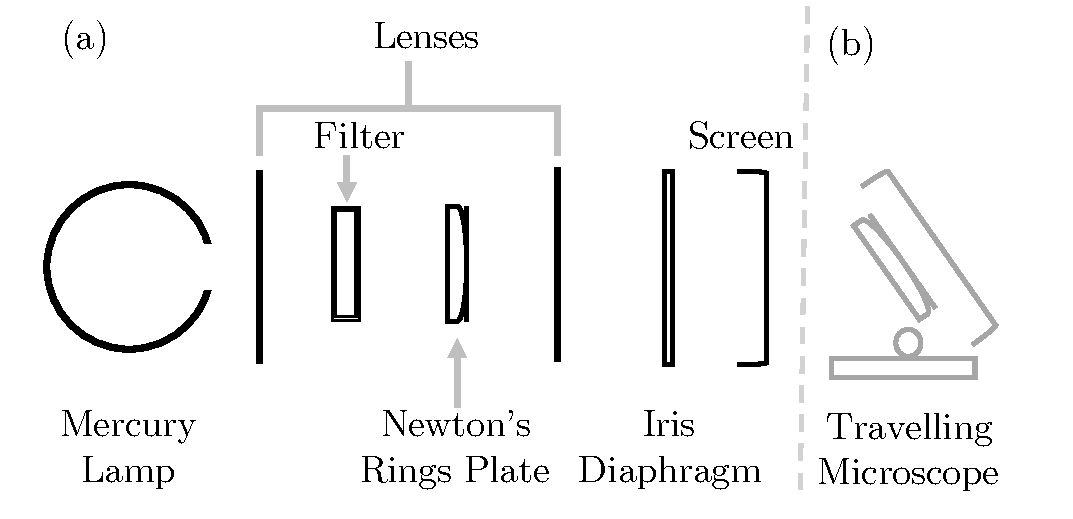
\includegraphics[width=9cm]{fig1}
\caption[]{(a) A schematic of the experimental set-up used to collect the initial set of data. Entire set-up was placed on an optical bench, allowing accurate positioning of the lenses.
\\
(b) Modified set-up used in subsequent investigations - Newton's Rings Plate is moved, the screen is adjusted, and a Travelling Microscope is added.}
\label{fig:fig1}
\end{center}
\end{figure}


The two main filters used varied by colour, yellow and green, this created the monochromatic light needed to view the interference fringes. It is worth noting that during the set-up the positions of the lenses and rings plate often had to be adjusted so that the pattern and the horizontal scale could be both focussed to the optimal level. An iris diaphragm was added to the setup so that there could be the greatest contrast between the light and dark fringes. Once this was done an initial measurement of the magnification was performed by comparing the distance of one of the projected tick-marks on the scale to the actual given value ($1$mm). 

Two sets of data were taken for each filter. In both cases the positions of the centre of the bright fringes along a horizontal axis were marked on a piece of paper attached to the screen. This was done only for the 10 innermost bright fringes as it gets progressively more difficult to distinguish the centres the further $m$ increases. The diameter was then measured for each fringe and a value for radius was obtained. A least squares fitting was applied to the fringe radius squared, $\rho_m^2$, along with $(m-1)\lambda$, where $m$ is the ring number and $\lambda$ is the wavelength of light used. For the yellow and green filters respectively, $\lambda_Y = (578\pm0.5)$ nm and $\lambda_G = (546 \pm 0.)5$ nm \cite{labscript}.

\vspace{-3ex}
\section{Results}
\vspace{-2ex}

The measured fringe radius squared, $\rho_m^2$, and $(m-1)\lambda$, is shown in Fig. 1. Through using a least squares fitting and equation (3) a value obtained for the radius of curvature, $R_{IE}$, turns out to be $15\pm3$m. 

In Table 1 we can see other values calculated for the radius of curvature from subsequent investigations using different methods but the same calculations. For example, taking measurements with a Travelling Microscope instead of direct screen measurements (see Fig. 1(b)) to measure the fringe radius. Moreover we repeated the initial experiment and collected additional data.  

Shown also in the table are values for $d_0$. 
\vspace{-1ex}
\begin{figure}[!h]
\begin{center}
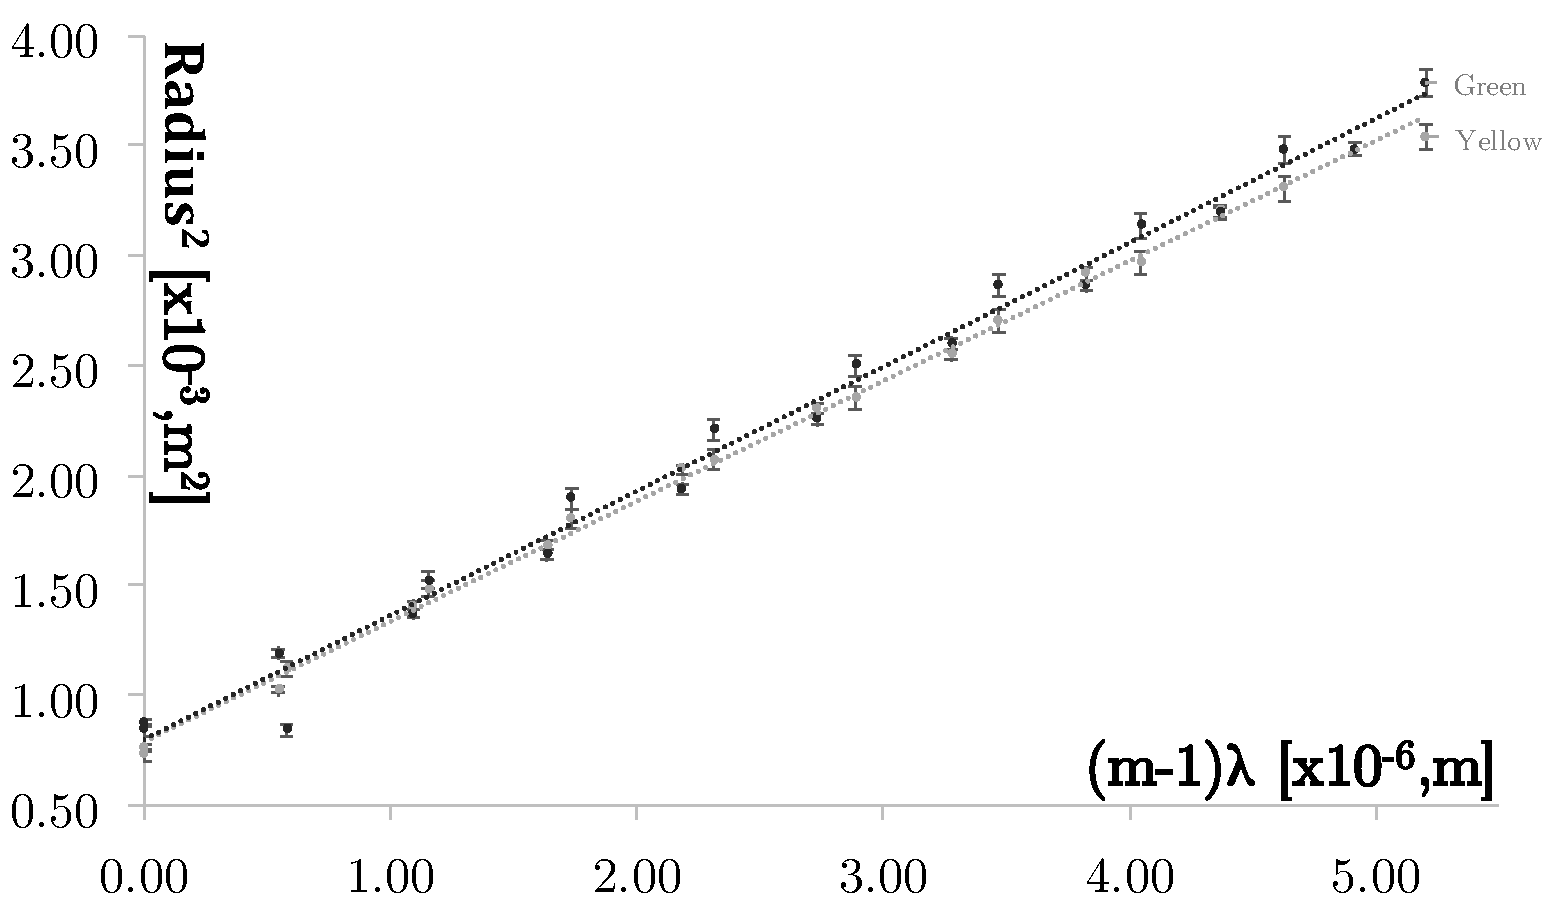
\includegraphics[width=9cm]{fig2}
\caption[]{The fringe radius squared plotted as a function of $(m-1)\lambda$. Horizontal error bars are too small to be seen.}
\label{fig:fig2}
\end{center}
\end{figure}


\begin{table}[h!]
\centering
\begin{tabular}{ |c|c|c|c| } 
 \hline
 \textbf{Experiment} & \textbf{Radius of Curvature, R $[m]$} & $\boldsymbol{d_0} [\times10^{-7}, m]$ \\ [0.5ex] 
 \hline\hline
 $IE$ &$15\pm3$ & $7\pm2$ \\ 
 %$[(m-1)\lambda]_{IE}$ & $R_{IE} = 15\pm3$ & $7\pm2$ \\ 
 %$(m-1)_{IE-Y}$& $16\pm2$ & - \\
 %\hline\hline
 $TM$ & $24\pm2$ & $4.6\pm0.9$ \\
 %$[(m-1)\lambda]_{TM}$ & $R_{TM} = 24\pm2$ & $4.6\pm0.9$ \\
 %$(m-1)_{TM-Y}$ & $21\pm2$ & - \\
 %$(m-1)_{TM-G}$ & $25\pm2$ & - \\
 %$(m-1)_{TM-B}$ & $28\pm1$ & - \\ 
 %\hline\hline
 $RE$ & $18\pm5$ & $8\pm3$ \\
 %$[(m-1)\lambda]_{RE}$ & $R_{RE} = 18\pm5$ & $8\pm3$ \\
 %$(m-1)_{RE-Y}$ & $18\pm3$ & - \\
 %$(m-1)_{RE-G}$ & $19\pm3$ & - \\
 %$(m-1)_{RE-B}$ & $26\pm5$ & - \\
 [1ex] 
 
 \hline
\end{tabular}
\caption{Values for radius of curvature of the planoconvex lens, and their respective values for $d_0$. IE denotes the 'Initial Experiment', TM for 'Travelling Microscope', and RE for 'Repeated Initial Experiment'.}
\label{table:1}
\end{table}

\vspace{-3ex}
\section{Discussion}
\vspace{-2ex}
In analysing our equipment we find that there are no official manufacturer's or literature value for the radius of curvature of the lens. We must compare the initial data and data collected in subsequent weeks of investigation in order to be able to draw some form of conclusion on what the radius of curvature should be. 

If we look at the plotted data in Fig. 2. we see that while the points do generally show the linear relationship between $\rho_m^2$ and $(m-1)\lambda$, more than half do not lie either on or within their respective trendlines with their uncertainties. This could be due to the fact that during data collection, the bright and dark fringes blur into one another so distinguishing where the centre of the bright fringe lay amounted to difficulty, this would inevitably lead to distances being incorrectly measured. Furthermore, random errors may have arisen due to varying eyesight and the interference pattern not being fully focussed, the former could be reduced by just having one person collecting data throughout. 

However, when we use this data to find a value for the radius of curvature, $R_{IE}=15\pm3$m, we at first doubt it's validity - the uncertainty is very large along with the actual value. But, after collecting data with a Travelling Microscope and using the same analysis, we get $R_{TM}=24\pm2$m, which is similar to $R_{IE}$. Given some consideration, we find that the large uncertainty could be due to how we measured the magnification, through measurement of only one of the projected tick-marks, if we had in fact measured ten of the distances individually, the uncertainty would have been reduced. 

\vspace{-0.5ex}

This is the case for the repeated experiment, $R_{RE}=18\pm5$, comparable values for the radius of curvature although the uncertainty has increased. This again could be due to magnification, a different value was used, $\times4$ instead of $\times6$ (noting $TM$'s $\times1$). 

There are a range of possible reasons for the differing values of $R$. For example, different filters were used in the investigations - what appeared to be the same colour each time could have been different. This would have lead to different wavelengths of monochromatic light being used. So the value for the radius of curvature would change accordingly, as can be seen by rearranging equation (3). This can also be caused by the non-perfect contact between the lens and glass plate, $d_0$. If the thickness of the film increases then the wavelength of the light in the film increases, so the radius of curvature will decrease.

We can see from Table 1 that when we used the Travelling Microscope set-up as shown in Fig. 1(b), the value for $d_{0-TM}$ is smaller than compared to $d_{0-IE}$ and $d_{0-RE}$. This could be due to the geometric path difference of the interfering light waves being changed. The value would be decreasing after being reflected at an angle from the screen thus resulting in a decrease of the value for $d_{0-TM}$. 

There are other ways in which the radius of curvature of a lens can be measured precisely using Newton's Rings. One is to use a digital camera and directly image the interference pattern produced - then digital software could be used to measure the fringe radius, avoiding any unnecessary random errors. On the other hand, we could coat the convex lens and the glass plate with high reflecting transparent silverings, this would allow the rings to appear sharper to avoid the issue of focussing the rings, moreover high precision also be attained here \cite{manchester}.

\vspace{-5ex}
\section{Conclusions}
\vspace{-2ex}
 
In conclusion, through measurements of Newton's Rings it has been possible to determine a value for the radius of curvature of a planoconvex lens, $R_{IE}=(15\pm3)$m. A value which at first was doubted, however after additional investigation it has been possible to compare and verify it is valid along with it's uncertainty. However, through modifying the experimental set-up it could be possible to reduce certain sources of uncertainties, and to remove some of the experimental issues experienced.

\begin{thebibliography}{5}
\bibitem{poiseuillehagen}
	Salvatore P. Sutera and Richard Skalak
	\textit{The History of Poiseuille's Law}.
	Annu. Rev. Fluid Mech., 1993.
	
\bibitem{collegephysics}
	Raymond A. Serway, Chris Vuille, and Jerry S. Faughin
	\textit{College Physics, 8th Edition}.
	Brooks/Cole, Belmont, CA, USA, 2009.

\bibitem{youngandfreedman} 
	Hugh D. Young and Roger A. Freedman.
	\textit{University Physics with Modern Physics, 13th Edition}. 
	Pearson Education Limited, Harlow, Essex, 2015.
	
\end{thebibliography}
\clearpage

\vfill
\twocolumngrid
\vspace{-3ex}
\section*{Appendix}
\vspace{-2ex}

The uncertainty calculated for the radius of curvature $R$ was found by propagating other uncertainties related to quantities found in equation (3). The majority of those uncertainties are calculated using equations based off formulae found in \textit{Measurements and their Uncertainties} [I. G. Hughes and T. P. A. Hase, \textit{Measurements and their Uncertainties}, Oxford University Press, Oxford, United Kingdom, 2010]. 
\\

Firstly for the square of the magnified radius of a bright fringe, $\rho_m^2$, the error is, 
\begin{equation} \tag{4}
\alpha_{r^2}=\alpha_r\abs{2\times r}
\end{equation}

where $r$ is the value for the magnified radius of a bright fringe, and $\alpha_r$ is it's respective uncertainty. In our experiment this value arises due to a 30 cm ruler being used to measure the diameter, so the highest precision achievable would have been limited at half a division, therefore $\alpha_r$=0.5 cm. 

The uncertainty on the magnification squared, $M^2$, is found by,
\begin{equation} \tag{5}
\alpha_{M^2}=M^2\abs{2\times\frac{\alpha_M}{M}}
\end{equation}

with $\alpha_{M}$ as the error on the magnification. For the initial and repeated experiment this value was taken to be $0.5$ due to the difficulties in measuring the width of one of the tick-marks with a $30$cm ruler. In the Travelling Microscope experiment $\alpha_{M}=0.005$ due to the precision to which we could measure with the vernier scale.    

To calculate the uncertainty on the radius of curvature $R$, the following equation is thus used,
\begin{equation} \tag{6}
\alpha_R=R\times\sqrt{\Big(\frac{\alpha_n}{n}\Big)^2 + \Big(\frac{\alpha_{M^2}}{M^2}\Big)^2 },
\end{equation}

where the term $n=(m-1)\lambda$, and the uncertainty on that, $\alpha_n$, was found by using a least squares fitting function in the software Microsoft\textregistered \ Excel. $M^2$ is again, the magnification squared with it's uncertainty $\alpha_{M^2}$ found above in equation (5).  

The uncertainty on $d_0$ is found by further propagating the uncertainties found above, the resulting equation is, 

\begin{equation} \tag{7}
\alpha_{d_0}=d_0\times\sqrt{\Big(\frac{\alpha_c}{c}\Big)^2 + \Big(\frac{\alpha_{M^2}}{M^2}\Big)^2 + \Big(\frac{\alpha_R}{R}\Big)^2}
\end{equation}

where $c$ is the intercept of the least squares fitting, and $\alpha_c$ is it's respective uncertainty.

With the case of the Travelling Microscope there is also the uncertainty on the vernier scale used, we shall take the highest precision it can measure to be $\alpha_{vernier}=0.5$mm.

\clearpage

%\footnotetext{I am not entirely too sure about what I did for (7), it was help from other students and the demonstrator}

\end{document}